\section{Available Kubernetes cluster deployment methods}
\textit{Here multiple methods of a Kubernetes cluster deployment are presented. Two chosen methods are described in a more detailed way. This is a theoretical chapter.}
\\

Kubernetes is \textbf{not trivial to deploy}. In order to deploy a usable cluster, there are at least two machines needed: one master and one node. On each of the machines several components must be installed. Apart from that, there are also requirements concerning networking to be met (described in section: \ref{k8s-net}) and a bunch of non-functional requirements (described in section: \ref{Production deployment requirements}) to be satisfied.

Fortunately, Kubernetes is a popular tool and many methods of deploying it are already described in the literature. The \textbf{available methods may be divided into three categories}:
\begin{itemize}
\item self-hosted solutions, on-premises,
\item deployment in a cloud, but not using Managed Services,
\item deployment in a cloud, using Managed Services.
\end{itemize}

Furthermore, different categorization may be applied. For instance, the deployment methods may be categorized \textbf{by the tools used}:
\begin{itemize}
\item using web interface of a particular cloud, e.g. AWS Management Console (supported by AWS),
\item using command-line tools officially supported by a particular cloud, e.g. awscli or eksctl (supported by AWS),
\item using command-line tools designed exactly to deploy a Kubernetes cluster, but not limited to one particular cloud, e.g. Kops,
\item using command-line tools tools, designed for managing computer infrastructure resources, e.g. Terraform, SaltStack.
\end{itemize}

There was an interesting study conducted by CNCF in 2019. A question was asked about \textbf{what tools are used in the respondents' organization or company to manage containers}. According to CNCF's Cloud Native Landscape, there are more than 109 such tools and 89\% of them are using different forms of Kubernetes. The \textbf{top 10 tools} are depicted on the following chart\cite{cncf-2019}. Based on this chart, it is observable that \textbf{the tool used the most often is Amazon Elastic Kubernetes Service (AWS EKS)} and the second most popular tool is Google Kubernetes Engine (GKE).

\begin{figure}[H]
    \centering
    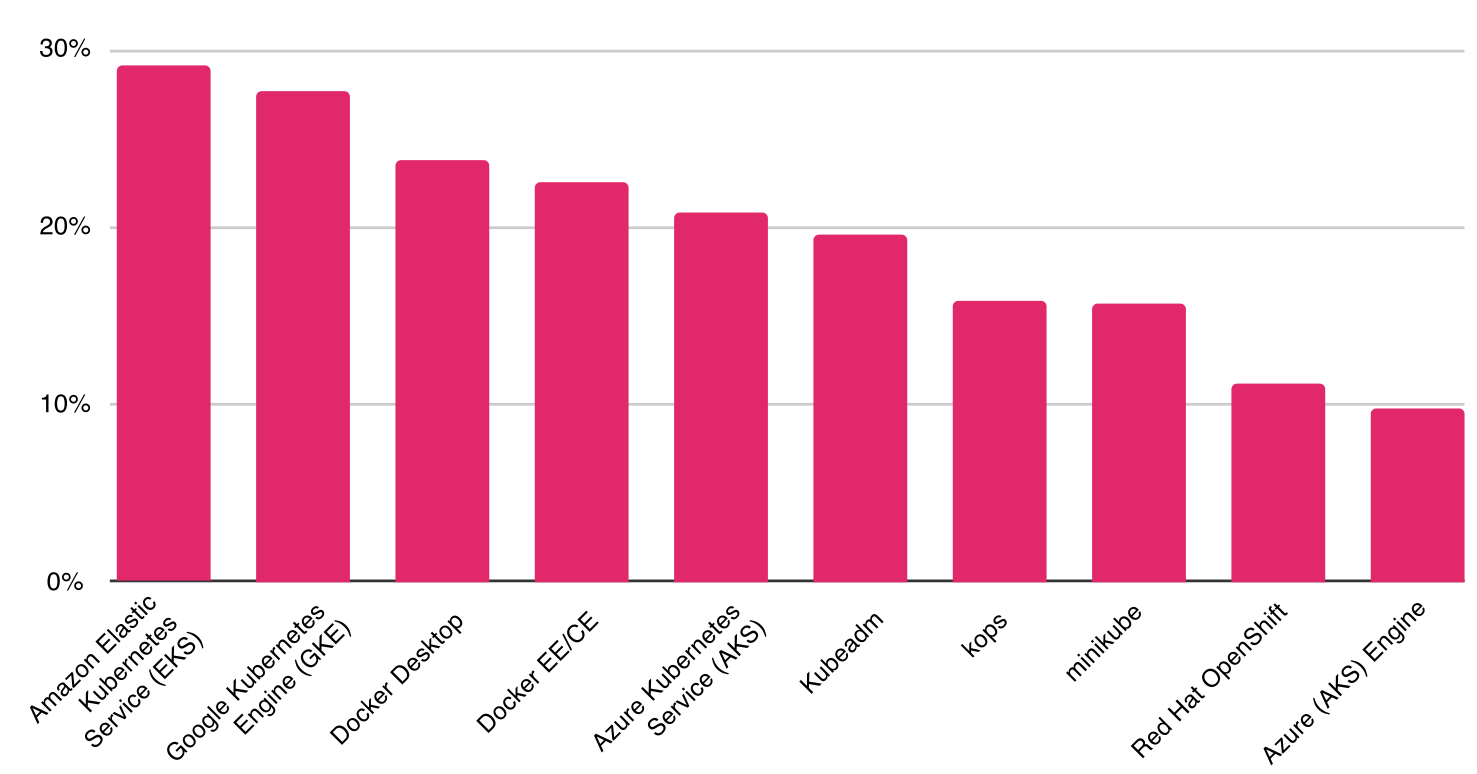
\includegraphics[width=16cm]{figures/cncf-2019-cont-tools.png}
    \captionsetup{justification=centering,margin=2cm}
    \caption{Top 10 tools used by organizations and companies to manage containers\cite{cncf-2019}}
\end{figure}

Further in this chapter, the methods categories (mentioned before) are briefly explained and a few methods are described in more detail. The focus is on \textbf{the two particular methods, which are used in the practical part of this work}:
\begin{itemize}
\item deploying on AWS, using AWS Managed Service (AWS EKS), using eksctl which is a AWS supported official tool,
\item deploying on AWS, not using any Managed Service, using Kops which is a command-line tool, not officially supported by any cloud, but designed exactly to deploy a Kubernetes cluster.
\end{itemize}

\subsection{Managed Services}
\textit{This section explains the term: Managed Services and lists some examples.}
\\

The complexity of Kubernetes infrastructure has a steep learning curve. Thus, a new market of services emerged: Managed Services. Managed Services are offered \textbf{to free the Kubernetes users of the burden of having to configure and maintain the not trivial Kubernetes infrastructure}. They provide a version of Kubernetes which is hosted and managed by a cloud\cite{article-managed}.

Managed services \textbf{offer a ready to use cluster}. The \textbf{popular Managed Kubernetes Services}, offered by major cloud providers, are:
\begin{itemize}
\item Elastic Kubernetes Service (Amazon EKS)\cite{online-eks}
\item Google Kubernetes Engine (GKE)\cite{online-gke}
\item Azure Kubernetes Service (AKS)\cite{online-aks}
\end{itemize}

\begin{figure}[H]
    \centering
    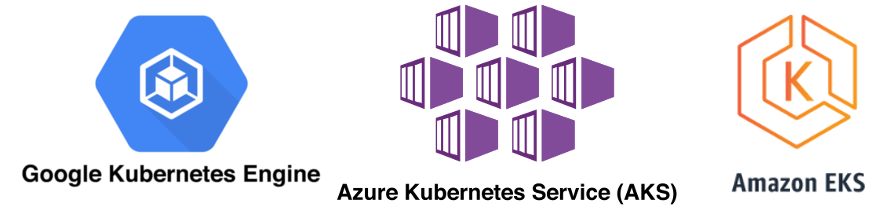
\includegraphics[width=10cm]{figures/managed-k8s.png}
    \captionsetup{justification=centering,margin=2cm}
    \caption{The logos of three Managed Kubernetes Services, offered by the major cloud providers}
\end{figure}

Managed Services are \textbf{deeply integrated with other resources offered by a particular cloud}. For example: AWS EKS is claimed to integrate with AWS services like: Amazon CloudWatch, Auto Scaling Groups, AWS Identity and Access Management (IAM), Amazon Virtual Private Cloud (VPC), and AWS App Mesh\cite{online-eks}. A nice feature of AKS is integrated continuous integration and continuous delivery (CI/CD) experience\cite{online-aks}. Moreover, GKE is advertised as offered with "integrated Cloud Monitoring with infrastructure, application, and Kubernetes-specific views"\cite{online-gke}.

\textbf{Managed Services are relatively new}. For example, the initial release of AWS EKS happened at 05.06.2018\cite{eks-history}. Thus, some literature may not acknowledge its existence, e.g. the book "Mastering Kubernetes"\cite{book-mastering-k8s}. Another effect of the Managed Services being so young is that, to the best of this work's author knowledge, there is no other formal study which compares the two chosen methods of Kubernetes cluster deployment, from a perspective of satisfying production environment requirements. There was, however, an interesting study conducted which compares three Managed Kubernetes Services (the three mentioned above: AWS EKS, AKS and GKE) from a performance perspective\cite{article-managed}.

\subsection{Command-line tools designed exactly to deploy a Kubernetes cluster}
\label{cli-tools-to-k8s}
\textit{In this section, several opensource command-line tools are discussed. These tools are not supported by any particular cloud provider, but they are designed exactly to fulfill one aim: to deploy a Kubernetes cluster.}
\\

Github.com is a popular (used by many people) website which hosts code repositories. Many of those repositories are opensource.  Github.com uses a star-rating system: whenever someone likes a particular project, one can give it a star. Thus, \textbf{the number of stars given to a project may be used as a popularity measure} of a particular project.

Searching through Github.com, there are several \textbf{command-line tools available which exist only to fulfill one aim: to deploy a Kubernetes cluster}. The names of a few of the most popular of these projects, together with the amount of stars they were acclaimed with, are presented on the image below.

\begin{figure}[H]
    \centering
    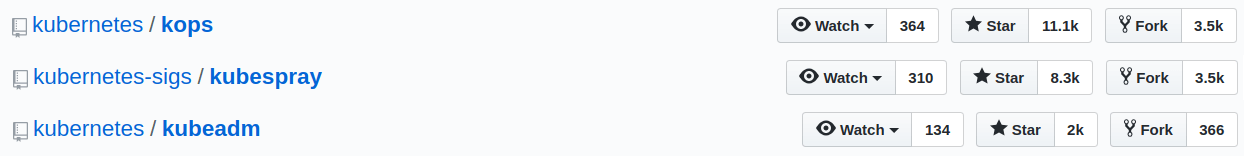
\includegraphics[width=17cm]{figures/custom-tools.png}
    \captionsetup{justification=centering,margin=2cm}
    \caption{Selected opensource tools which deploy a Kubernetes cluster, found on Github.com, state for date: 20.04.2020}
\end{figure}

The most popular tool amongst the four above is: \textbf{Kops}. Kops stands for Kubernetes Operations and on its Github.com page it is advertised as "the easiest way to get a production grade Kubernetes cluster up and running"\cite{online-kops-gh}. It is a command-line tool which allows to create, destroy, upgrade and maintain production-grade, highly available, Kubernetes clusters. It supports multiple clouds: AWS (officially), GCE and OpenStack (in beta support) and VMware vSphere (in alpha)\cite{online-kops-gh}. Furthermore, it can be used from multiple operating systems: Linux, Mac and Windows\cite{online-kops-install}. Kops is one of the recommended ways to setup a Kubernetes cluster and it is a tool which can be used to a create a producttion environment\cite{book-devops-with-k8s}

The second most popular tool is \textbf{Kubespray}. It also supports multiple clouds: AWS, GCE, Azure, OpenStack, vSphere, Oracle Cloud Infrastructure (Experimental), and Baremetal\cite{online-ks}. Furthermore, it also supports Highly Available deployment. The main difference between Kubespray and Kops is that \textbf{Kubespray uses Ansible} (an opensource tool to provision infrastructure) while \textbf{Kops performs the provisioning and orchestration itself}. Kops also provides more features tightly integrated with specified clouds\cite{online-ks-comp}.

There is also \textbf{kubeadm}. In contrast to Kops and Kubespray, kubeadm helps to get a minimum viable cluster "in a user friendly way". Furthermore, its scope is limited to the local filesystem\cite{online-kubeadm}. Kubernetes (and kubeadm) maintainers state that kubeadm is supposed to become a building block for all Kubernetes deployments. They also want to identify the common phases of a cluster deployment and make kubeadm an easy-to-use and configurable set of commands for each of those phases. An example of a common phase could be: certificate distribution\cite{kubeadm-vision-2017}.

Other than these three briefly described tools, \textbf{there are many more}, for instance: kube-aws\cite{kube-aws} or minikube\cite{minikube}. But neither listing them all nor describing them is needed for the purpose of this work. In the empirical part of this work, only one of the described tools is used: Kops.

\subsection{Custom solutions}
\textit{In this section, custom solutions for a Kubernetes cluster deployment are presented.}
\\

There is always a way to do (almost) everything on one's own. Here, one can split the deployment into two phases: infrastructure creation and, then, provisioning. To create infrastructure, meaning: virtual machines (compute resources), network and storage resources, one can use the following tool: \textbf{Terraform}. It is a tool made by Hashicorp, which incorporates \textbf{Infrastructure as Code}, in order to manage infrastructure. It has a CLI and thus it is fairly easy to use with a Continuous Integration server. Thanks to declarative configuration files, the resultant infrastructure is easy to reproduce\cite{terraform}. IaC facilitates future repetition of any work done with Terraform and thus any evaluations of this tool (done by experimenting with it) may be repeated in the future.

Terraform supports many providers, meaning that it can manage infrastructure of different public and private clouds (like: AWS, GCP, Azure, OpenStack) and, it can also handle local operations\cite{terraform}. There are also some alternative solutions, e.g.: \textbf{Heat or CloudFormation}. They support declarative configuration files too. But they are not cloud-agnostic. Heat is a solution for OpenStack cloud and CloudFormation - for AWS. Sometimes, there is a need to use many various providers in order to build an infrastructure and then, one may view it as a nice feature, to be able to use a unified syntax, which Terraform provides\cite{terraform-vs}.

After the infrastructure is created, the next step is to provision it. This step involves installing needed software (in this case: Kubernetes) and configuring it. However, since Kubernetes cluster is not just one machine, it would be tremendously tedious to provision each machine one by one manually. Thus, a chosen Configuration Management tool should be applied. There are any opensource tools available, some have been already presented in the section: \ref{Automation as production environment requirements}.

There was a time, when \textbf{Kubernetes source code contained SaltStack code}, in order to provision a cluster. The code can be still found on github: \url{https://github.com/kubernetes/kubernetes/tree/release-0.13/cluster/saltbase/salt}. However, now this method is deprecated (as can be read e.g. on this page: \url{https://github.com/kubernetes/kubernetes/tree/v1.18.2/cluster/}).

The advantage of such a custom solution is that it is very customizable and that, by making it work, one can learn Kubernetes in depth. On the other hand, it is not nearly as fast to design and first run as Managed Services. If one would like to immerse into the ocean of Kubernetes knowledge base, another great idea could be to try Kubernetes The Hard Way\cite{k8s-thw}.


\subsection{Deployment method: on AWS EKS Managed Service using eksctl}
\textit{Here is briefly described the first of the two methods, which are used in the empirical part of this work.}
\\

The goal of this method is to have the Kubernetes control plane managed by AWS. This means that it is AWS which is responsible for managing Kubernetes master components, such as: API Server, kube-scheduler, kube-controller-manager and also Etcd. The \textbf{control plane should be already highly available}, thanks to being deployed across \textbf{multiple Availability Zones}\cite{what-is-eks}. Availability Zone (AZ) is an isolated geographically place to host Amazon data centers. Several AZs create a Region. AZs in a Region are connected through low-latency links\cite{az}.

The control plane being already highly available means that there should be at least two API server nodes and three etcd nodes that run across three Availability Zones within a Region. In addition, AWS EKS is responsible for automatically detecting and replacing unhealthy control plane instances. Furthermore, version upgrades should be provided automatically and applied\cite{what-is-eks}. There exists a \textbf{Service Level Agreement (SLA)} especially concerning AWS EKS. It is a policy which governs the use of the Amazon Elastic Container Service for Kubernetes. For example, the SLA states what is the Monthly Uptime Percentage during any monthly billing cycle (at least 99.95\%)\cite{eks-sla}. Thanks to such a SLA, AWS EKS is claimed to be \textbf{reliable and recommended for production workloads}\cite{what-is-eks}.

Furthermore, AWS EKS also manages the Kubernetes (worker) nodes. The nodes are run in one's AWS account and AWS connects them to the already deployed control plane via the cluster API server endpoint. The worker nodes are grouped in an AWS EC2 Auto Scaling group. The latter fact has some consequences, namely all these nodes have to\cite{eks-worker}:
\begin{itemize}
\item use the same Amazon EC2 instance type,
\item be instantiated from the same Amazon EC2 image (called: AMI, an abbreviation from Amazon Machine Image\cite{aws-ami}),
\item use the same Amazon EKS worker node IAM role.
\end{itemize}

Fortunately, an AWS EKS cluster can contain multiple node groups, therefore there is a possibility to utilize nodes of various AMIs\cite{eks-worker}. This is an important information, because a Kubernetes administrator may be interested in choosing a particular operating system for a node. There exist such AMIs, which are specifically designed for EKS. This AMI is built on top of Amazon Linux 2 and has some essential tools installed and configured: Docker, kubelet, and the AWS IAM Authenticator. The way in which the AMI is built is coded and made opensource. Thanks to this solution, everyone can build their own AMI, basing on the opensource version\cite{eks-optimized-ami}. There is even an option to have Windows worker nodes\cite{eks-worker-win}.

The cluster control plane is fronted by \textbf{an Elastic Load Balancing Network Load Balancer} and also all the networking is taken care of (elastic network interfaces are provisioned in VPC subnets) to provide connectivity from the control plane instances to the worker nodes. Thanks to that, the AWS EKS \textbf{user can access the Kubernetes API Server}\cite{eks-clusters}.

In order to use AWS EKS, there are two ways supported:
\begin{itemize}
\item using eksctl CLI,
\item using AWS Management Console and AWS CLI.
\end{itemize}

Both of them demand installing AWS CLI. In this work, \textbf{the method with eksctl CLI is applied}. Eksctl is officially the CLI for AWS EKS, endorsed by AWS, though it was launched by WeaveWorks. With eksctl, one can use a simple command to instantiate the whole cluster\cite{eks-cli-official}:
\begin{lstlisting}[basicstyle=\small,caption={A command of eksctl CLI tool used to create a Kubernetes cluster},captionpos=b,language=Bash,xleftmargin=1cm]
$ eksctl create cluster
\end{lstlisting}

The cluster can be \textbf{configured with a YAML file and also by setting eksctl CLI flags}. The documentation describing how to do it, is presented on the official eksctl website\cite{eksctl}. There is also an example YAML configuration file attached on that website. This file is used to customize a cluster. It is also appended below.

\begin{lstlisting}[basicstyle=\tiny,caption={An example YAML file used to customize a Kubernetes cluster created with eksctl CLI tool\cite{eksctl}},captionpos=b,language=Bash,xleftmargin=1cm]
apiVersion: eksctl.io/v1alpha5
kind: ClusterConfig

metadata:
  name: basic-cluster
  region: eu-north-1

nodeGroups:
  - name: ng-1
    instanceType: m5.large
    desiredCapacity: 10
  - name: ng-2
    instanceType: m5.xlarge
    desiredCapacity: 2
\end{lstlisting}

This example configuration file sets a name for the cluster ('basic-cluster'), chooses an Amazon Region in which all the AWS resources will be deployed ('eu-north-1') and also configures the details of Kubernetes nodes. Many more options can be set.

After the cluster is created and after a connectivity with a Kubernetes cluster endpoint is established, it is now possible to deploy applications on top of the cluster. The illustration below depicts the stages of working with AWS EKS.
\begin{figure}[H]
    \centering
    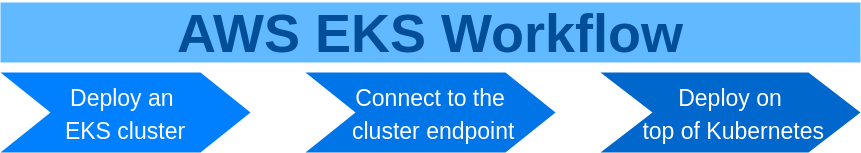
\includegraphics[width=12cm]{figures/eks-workflow.png}
    \captionsetup{justification=centering,margin=2cm}
    \caption{A schema presenting the stages of working with AWS EKS}
\end{figure}

Much more information on how to deploy AWS EKS Kubernetes cluster can be found. The official websites of AWS EKS\cite{what-is-eks} and eksctl\cite{eksctl} are a great source of help. More examples of cluster configuration can be found on the official eksctl page on Github.com\cite{eks-gh}. A sample Kubernetes use cases scenarios, for example: creating a CI pipeline to deploy a sample Kubernetes service, can be found in the Internet\cite{eksworkshop}.


\subsection{Deployment method: on AWS using Kops}
\textit{Here is briefly described the second of the two methods, which are used in the empirical part of this work.}
\\

Kops was already introduced in the section: \ref{cli-tools-to-k8s}. Similarly to eksctl, Kops can also create a Highly Available Kubernetes cluster. However it demands more work than eksctl. The commands which allow to create a cluster on AWS is\cite{book-mastering-k8s}:
\begin{lstlisting}[basicstyle=\small,caption={The commands of Kops CLI tool used to create a Kubernetes cluster},captionpos=b,language=Bash,xleftmargin=1cm]
$ kops create cluster --cloud=aws --zones=us-east-1c ${NAME}
\end{lstlisting}
But, before these commands can be run, one has to provide some minimal DNS configuration via Route53 (an AWS resource responsible for networking), set up a S3 bucket (another AWS resource, responsible for storage) to store the cluster configuration\cite{book-mastering-k8s} and also configure the AWS IAM user (an AWS resource responsible for access management) and create a SSH key pair\cite{online-kops-aws}. The instructions explaining how to set up the AWS resources are provided on the official Kops website\cite{online-kops-aws}.

The configuration of Kops is kept in an S3 bucket. In order to change the configuration, one has to enter the following command\cite{online-kops-aws}:
\begin{lstlisting}[basicstyle=\small,caption={A command of Kops CLI tool used to edit a Kubernetes cluster configuration},captionpos=b,language=Bash,xleftmargin=1cm]
$ kops edit cluster ${NAME}
\end{lstlisting}

A configuration spec file is generated during the create phase and uploaded to a S3 bucket. The configuration can be also kept in YAML file. All the configuration options are available on a Kops Golang documentation website\cite{online-kops-yaml-config-golang}. A cluster can be created then in the following way\cite{online-kops-yaml-config}:
\begin{lstlisting}[basicstyle=\small,caption={A command of Kops CLI tool used to create a Kubernetes cluster using a YAML configuration file},captionpos=b,language=Bash,xleftmargin=1cm]
$ kops create -f $NAME.yaml
\end{lstlisting}


The stages of working with a Kubernetes cluster deployed on AWS with Kops are similar to the stages of working with eksctl, but there is the additional first stage. It is depicted on the below schema.
\begin{figure}[H]
    \centering
    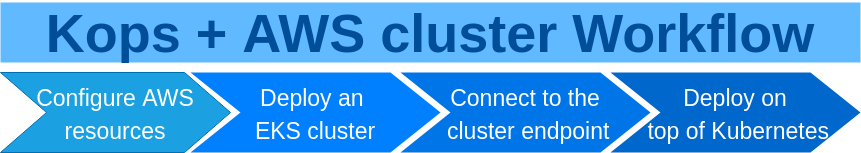
\includegraphics[width=12cm]{figures/kops-aws-workflow.png}
    \captionsetup{justification=centering,margin=2cm}
    \caption{A schema presenting the stages of working with a Kubernetes cluster deployed on AWS with Kops}
\end{figure}

The next stage, after instantiating a cluster is to connect to it through an endpoint. Such configuration is automatically generated and written to '~/.kube/config' (on Linux Operating System)\cite{online-kops-aws}. The same is true also for AWS EKS.

Kops has been around a long time as an AWS-specific tool, but now it also supports other clouds\cite{book-cndwk}\cite{online-kops-gh}. Its main features such as: automated Kubernetes cluster deployment, highly available master or adding a variety of custom Kubernetes addons\cite{kops-addons} indicate that Kops is an attractive tool, worthy to at least try out.

There are many Internet sources available to broaden one's knowledge about Kops: the official Kops website\cite{online-kops}, the Kops project website on Github.com\cite{online-kops-gh} and there are also some comparisons of Kops versus alternative tools available, e.g.: "A Multitude of Kubernetes Deployment Tools: Kubespray, kops, and kubeadm"\cite{online-kops-blog}.

\subsection{Amazon services allowing to run containers}
\textit{In order to exhaust the topic of the Amazon services which allow to run containers, this chapter was created. This chapter shortly characterizes each such AWS Service.}
\\

Below, all the AWS Services, used to manage containers, are listed:
\begin{itemize}
\item AWS ECS
\item AWS ECR
\item AWS Fargate
\item AWS EKS
\end{itemize}

\textbf{AWS ECS} stands for Amazon Elastic Container Service. It is a service that provides \textbf{a highly secure, reliable, and scalable way to run containers}. Secure, because the containers are run in a custom VPC (Virtual Private Cloud). Thanks to that, custom firewall rules can be applied to the containers (by using AWS Security Groups). Furthermore, each of the containers uses IAM, which means that access to each container can be restricted and granular access permissions can be assigned. Running containers on ECS is reliable thanks to the SLA, which guarantees a Monthly Uptime Percentage of at least 99.99\%\cite{ecs}.

\textbf{AWS ECR} is an abbreviation from Amazon Elastic Container Registry. It is not a service which strictly manages the containers, but it manages images. It is \textbf{a fully-managed Docker container registry}. AWS ECR eliminates the need to run such a registry on-premises or worry about scaling the underlying infrastructure. The images are hosted in a highly available and scalable architecture. Similarly to AWS ECS, AWS ECR also integrates with IAM\cite{ecr}.

\textbf{AWS Fargate is a serverless service to run containers}. This service is responsible for allocating the right amount of compute, eliminating the need to choose instances and scale cluster capacity. It can work with both: AWS ECS and AWS EKS. AWS Fargate runs each task or pod in its own kernel, therefore the tasks and pods are provided with their own isolated compute environment. Without Fargate, the containers are run on EC2 instances, so the end user has to pay for both: an EC2 instance and for an ECS container\cite{fargate}. Running serverless Kubernetes Pods Using Amazon EKS and AWS Fargate is very new, a blog post informing about this possibility was created at 3rd of December 2019\cite{fargate-for-eks}.

The last service on the list above, \textbf{AWS EKS}, was already described in this chapter.

\subsection{Summary}

There are \textbf{many methods of deploying a Kubernetes cluster}. According to the authors of "Cloud Native DevOps with Kubernetes"\cite{book-cndwk}, the best solution is to use \textbf{Managed Services}. The authors argue that, thanks to this method, one can get a fully working, secure, highly available, production-grade cluster in a few minutes and for a little price. Managed Services are certainly a good way to try Kubernetes out. Then, if one wants to do something non-standard or to experiment with the cluster, then one could choose \textbf{a custom or a hybrid solution}. The self-hosted, deployed on-premises way is recommended if the following qualities are of a great importance: price, low-network latency, regulatory requirements and total control over hardware\cite{book-mastering-k8s}.

Managed Services offer many features like: built-in autoscaling, security, high availability, having serverless options. However, they may be more expensive (for example, when using AWS EKS, one has to pay \$0.10 per hour for each Amazon EKS cluster\cite{online-eks-pricing}) and less customizable. Custom solutions allow the Kubernetes administrator to broaden their knowledge and \textbf{grasp the deep understanding} on what is going on under the Kubernetes hood (i.e. one can customize how the Kubernetes control plane is deployed or set up a custom network topology).

There is \textbf{no one right answer} which fits all the use cases. It is always advised to do one's own research and to try and experiment with the existing methods.
